\section{Theory}

Frequency-selective or filter circuits pass only those input signals to the output that are in a desired range of frequencies (called \textit{pass band}). The amplitude of signals outside this range of frequencies (called \textit{stop band}) is reduced (ideally to zero). The frequency between pass and stop bands is called the \textit{cut-off frequency} ($\omega_c$). 

Typically in these circuits, the input and output currents are kept to a small value and as such, the current transfer function is not an important parameter. The main parameter is the voltage transfer function in the frequency domain or \textit{gain}, given by $H_v$ or $H(j\omega) = V_o/V_i$. As $H(j\omega)$ is complex number, it has both a magnitude and a phase. Filters in general introduce a phase difference between input and output signals.

\subsection*{RC Filters}

The simplest passive filter circuit can be made by connecting together a single resistor and a single capacitor in series across an input signal, ($V_i$) with the output signal, ($V_o$) taken from the junction of these two components. Depending on which way around we connect the resistor and the capacitor with regards to the output signal determines the type of filter construction resulting in either a Low Pass or a High Pass Filter. As there are two passive components within this type of filter design the output signal has amplitude smaller than its corresponding input signal, therefore passive RC filters attenuate the signal and have a gain of less than one.

Additionally in practical filters, pass and stop bands are not clearly defined, as $|H(j\omega)|$ varies continuously from its maximum towards zero. The cut-off frequency is, therefore, defined as the frequency at which $|H(j\omega)|$ is reduced to $1/\sqrt{2}$ of its maximum value. This corresponds to signal power being reduced by $1/2$ as $P \propto V^2$.

\subsection{Low Pass Filters}

A low pass filter or LPF attenuates or rejects all high frequency signals and passes only low frequency signals below its characteristic frequency called as cut-off frequency, $\omega_c$. An ideal low-pass filter's transfer function is shown in Fig. 1(a).

\begin{figure}[H]
    \centering
    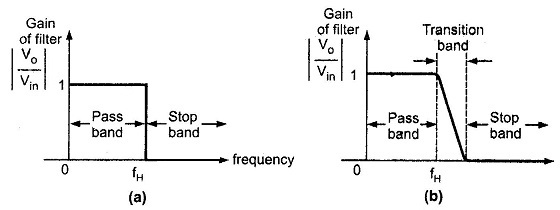
\includegraphics[width=1\columnwidth]{images/f5.jpg}
    \caption{Transfer functions of an (a) ideal and a (b) practical low-pass filter}
    \label{fig:1}
\end{figure}

In practical terms, a series RC circuit can act as a low pass filter. For no load resistance (output is an open circuit, $R \rightarrow \infty$),

\begin{align}
    V_o = \frac{1/(j\omega C)}{R+1/(j\omega C)}V_i &= \frac{1}{1+j\omega RC}V_i\\
    H(j\omega) = \frac{V_o}{V_i} &= \frac{1}{1+j\omega RC}
\end{align}

where $X_C = 1/(j\omega C)$ is the impedance of the capacitor. To find the cut-off frequency ($\omega_c$), we note,

\begin{align}
    |H(j\omega)| = \frac{1}{\sqrt{1+(\omega RC)^2}}
\end{align}

When $\omega \rightarrow 0$, $|H(j\omega)| \rightarrow 1$ is maximum. For $\omega = \omega_c$, $|H(j\omega)| = 1/\sqrt{2}$. Thus,

\begin{align}
    |H(j\omega)| &= \frac{1}{\sqrt{1+(\omega_c RC)^2}} = \frac{1}{\sqrt{2}}\\
    \implies \omega_c &= \frac{1}{RC}\\
    \text{So, } |H(j\omega)| &= \Bigg|\frac{1}{1+\frac{j\omega}{\omega_c}}\Bigg| = \frac{1}{\sqrt{1+\left(\frac{\omega}{\omega_c}\right)^2}} \\
    \text{and phase, } \phi &= -\taninv{\frac{\omega}{\omega_c}}
\end{align}

\paragraph*{\textbf{Input Impedance}}

\begin{align*}
    Z_i = R+\frac{1}{j\omega C}
\end{align*}

The value of the input impedance depends on the frequency $\omega$. For good voltage coupling, we need to ensure that the input impedance of this filter is much larger than the output impedance of the previous stage. Thus, the minimum value of $Z_i$ is an important number. $Z_i$ is minimum when the impedance of the capacitor is zero ($\omega \rightarrow \infty$), i.e. $Z_i\big|_\text{min} = R$. \\

\paragraph*{\textbf{Output Impedance}}
The output impedance can be found by shorting the source and finding the equivalent impedance between output terminals,

\begin{align*}
    Z_o = R \bigg|\bigg|  \frac{1}{j\omega C}
\end{align*}

where the source resistance is ignored. Again, the value of the output impedance also depends on the frequency $\omega$. For good voltage coupling, we need to ensure that the output impedance of this filter is much smaller than the input impedance of the next stage, the maximum value of $Z_o$ is an important number. $Z_o$ is maximum when the impedance of the capacitor is $\infty$ ($\omega \rightarrow 0$), i.e. $Z_o\big|_\text{max} = R$.

\subsubsection*{\textbf{Bode plots}}
The ratio of output to input power in a two-port network is usually expressed in decibels,

\begin{align*}
    |H(j\omega)|_\text{dB} = 10\log_{10}\left(\frac{P_o}{P_i}\right) = 20\log_{10}\left(\frac{V_o}{V_i}\right)
\end{align*}

\begin{figure}[H]
    \centering
    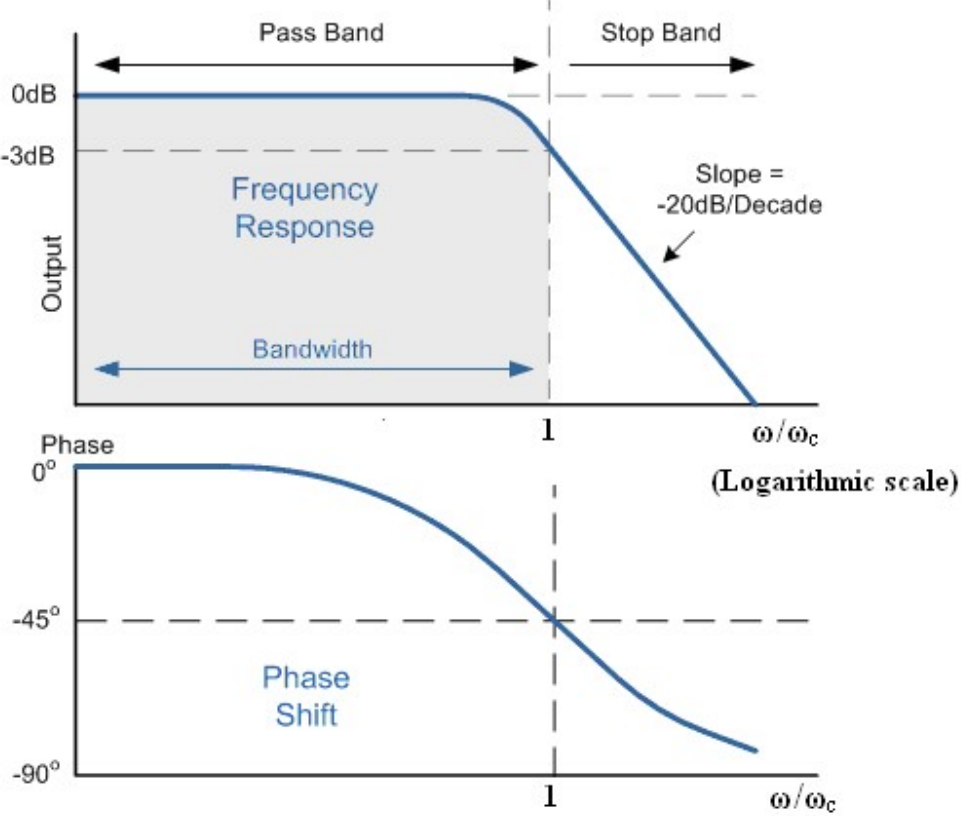
\includegraphics[width=1\columnwidth]{images/f7.png}
    \caption{Bode Plots for low-pass RC filter}
    \label{fig:2}
\end{figure}

At high frequencies, $\omega/\omega_c>>1$, $|H(j\omega)| \approx 1/(\omega/\omega_c)$ and $|H(j\omega)|_\text{dB} = 20\log(\omega_c)-20 \log(\omega)$, which is a straight line with a slope of -20 dB/decade in the Bode plot. It means that if $\omega$ is increased by a factor of 10 (a decade), $|H(j\omega)|_\text{dB}$ changes by -20 dB. Here, $\phi \approx 0^{\circ}$

At low frequencies $\omega/\omega_c<<1$, $|H(j\omega)| \approx 1$, which is also a straight line in the Bode plot. Here, $\phi \approx 90^{\circ}$

The intersection of these two \textit{asymptotic} values is at $1 =  1/(\omega/\omega_c)$ or $\omega = \omega_c$ . Because of this, the cut-off frequency is also called the \textit{corner} frequency.

One can see that there is a 3 dB difference between maximum gain and gain at the cut-off frequency,

\begin{align*}
    20\log|H(j\omega_c)|&-20\log|H(j\omega)|_\text{max}\\
    = 20\log \frac{|H(j\omega_c)|}{|H(j\omega)|_\text{max}} &= 20\log\frac{1}{\sqrt{2}} = -3 \text{ dB}
\end{align*}

\subsection{High Pass Filters}

A high pass filter, is the exact opposite of the LPF circuit. It attenuates or rejects all low frequency signals and passes only high frequency signals above $\omega_c$.

\begin{figure}[H]
    \centering
    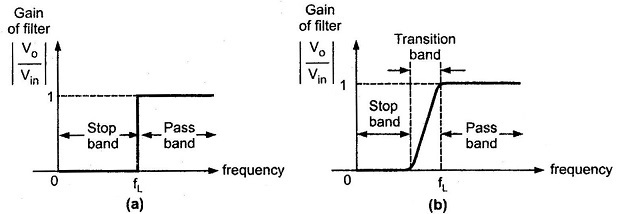
\includegraphics[width=1\columnwidth]{images/f6.jpg}
    \caption{Transfer functions of an (a) ideal and a (b) practical high-pass filter}
    \label{fig:3}
\end{figure}

In practical terms, a series RC circuit can also act as a high pass filter. For no load resistance (output is an open circuit, $R \rightarrow \infty$),

\begin{align}
    V_o = \frac{R}{R+1/(j\omega C)}V_i &= \frac{1}{1-j(1/\omega RC)}V_i\\
    H(j\omega) = \frac{V_o}{V_i} &= \frac{1}{1-j(1/\omega RC)}
\end{align}

The gain of this filter, $|H(j\omega)|$ is maximum ($=1$) when $\omega \rightarrow \infty$. Thus, the cut-off frequency can be found by,

\begin{align}
    |H(j\omega)| &= \frac{1}{\sqrt{1+(1/\omega_c RC)^2}} = \frac{1}{\sqrt{2}}\\
    \implies \omega_c &= \frac{1}{RC}\\
    \text{So, } |H(j\omega)| &=  \frac{1}{\sqrt{1+\left(\frac{\omega_c}{\omega}\right)^2}} \\
    \text{and phase, } \phi &= \taninv{\frac{\omega_c}{\omega}}
\end{align}

\paragraph*{\textbf{Input Impedance}}
\begin{align*}
    Z_i = R+\frac{1}{j\omega C} \text{ and } Z_i\big|_\text{min} = R
\end{align*}

\paragraph*{\textbf{Output Impedance}}
\begin{align*}
    Z_o = R\bigg|\bigg|\frac{1}{j\omega C} \text{ and } Z_i\big|_\text{max} = R
\end{align*}

\subsubsection*{\textbf{Bode plots}}

\begin{figure}[H]
    \centering
    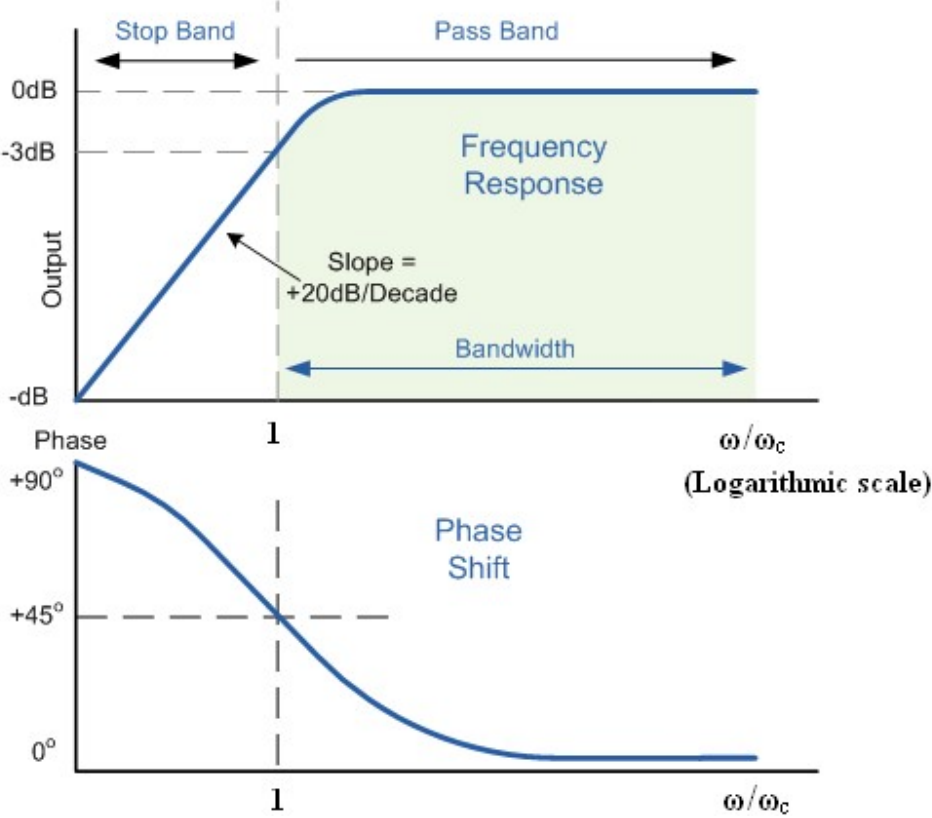
\includegraphics[width=1\columnwidth]{images/f8.png}
    \caption{Bode Plots for high-pass RC filter}
    \label{fig:4}
\end{figure}

At high frequencies, $\omega/\omega_c>>1$, $|H(j\omega)| \approx 1$, which is a straight line with a slope of 0 dB/decade in the Bode plot. Here, $\phi \approx 90^{\circ}$.

At low frequencies $\omega/\omega_c<<1$, $|H(j\omega)| \propto \omega$, which is a straight line with a slope of +20 dB/decade in the Bode plot. Here, $\phi \approx 0^{\circ}$.

\subsection*{Applications}
Filter circuits are used in a wide variety of applications. High-frequency band-pass filters (several hundred MHz) are used for channel selection in telephone central offices. 

Data acquisition systems usually require anti-aliasing low-pass filters as well as low-pass noise filters in their preceding signal conditioning stages. They are also used as to reduce any low frequency noise or “rumble” type distortion in speaker systems.

In the field of telecommunication, band-pass filters are used in the audio frequency range (20 Hz to 20 kHz) for modems and speech processing. System power supplies often use band-rejection filters to suppress the 50 Hz line frequency and high frequency transients.